\section{Achieving conflict-freedom in POSIX}

Given that many commutative operations are not conflict-free in Linux,
is it feasible to build file system and virtual memory systems that
do achieve conflict-freedom?
%
To answer this
question, we designed and implemented a \code{ramfs}-like in-memory
file system called \fs and a virtual memory system called RadixVM for
\sys, our research kernel based on xv6~\cite{xv6}.
%
Although it is in principle possible to make the same changes in Linux,
we chose not to implement \fs in Linux because \fs's design
would have required extensive changes throughout the Linux kernel.
%
The designs of both RadixVM and \fs were guided by the
commutativity rule.  For \fs, we relied heavily on \tool throughout
development to guide its design and identify sharing problems in its
implementation.  RadixVM
was built prior to
\tool, but was guided by manual reasoning about commutativity and
conflicts, which we later validated using \tool.

\begin{figure*}
\small
\centering
\inputnodraft{figures/testcases-sv6}
\caption{Conflict-freedom of commutative system call pairs in \sys.}
\label{fig:testcase-breakdown-sv6}
\end{figure*}

\Cref{fig:testcase-breakdown-sv6} shows the result of applying \tool
to \sys.  In contrast with Linux, \sys is conflict-free for nearly
every commutative test case.  The rest of this chapter explores how we
accomplish this in \sys to answer the following questions:

\begin{CompactItemize}

\item What techniques are necessary to achieve scalability for
      cases where current file and virtual memory systems do not
      scale?

\item What situations might be too difficult or impractical to
      make scale, despite being commutative?

\end{CompactItemize}

This chapter starts with the design of Refcache, a scalable reference
counting mechanism used throughout \sys.  It then covers the designs
of RadixVM and \fs.  Finally, it discusses operations that are
difficult to make conflict-free without sacrificing other practical
concerns.

\subsection{Refcache: Conflict-free reference counting}

\XXX![AC]{This is verbatim from the (corrected) EuroSys paper.  Update
  to fit.}

Reference counting is critical to many OS functions, and \vm is no
different.  Since two virtual memory regions may share the same physical
pages, such as when forking a process, \vm must have a way
to decide when to free the underlying physical pages.  To do so,
\vm reference counts each physical page, but a simple scheme with a
single counter can result in scalability problems because threads will
contend for the counter.  Likewise, \vm reference counts nodes of its
radix tree to determine when they are empty; a single counter would
cause operations on different parts of the node to contend.

This section introduces \refcache, a novel
reference counting scheme that \vm uses to track and reclaim physical
memory pages and radix tree nodes.
\refcache implements space-efficient, lazy, scalable reference
counting using per-core \emph{reference delta caches}.  \refcache targets
workloads that can tolerate some latency in reclaiming resources and
where increment and decrement operations often occur on the same core
(e.g., the same thread that faulted pages into a mapped memory region
also unmaps that region).  

In contrast with most scalable
reference counting mechanisms (see \S\ref{sec:related}), \refcache
requires space proportional to the sum of the number of reference
counted objects and the number of cores, rather than the product, and
the per-core overhead can be adjusted to trade off space and
scalability by controlling the reference delta cache conflict rate.  This is
important when tracking every physical page in a large multicore
system; at large core counts, typical scalable reference counters
would require more than half of physical memory just to track the
remaining physical memory.  

\refcache batches increment and decrement
operations, reducing cache line movement while offering an adjustable
time bound on when an object will be garbage collected after its
reference count drops to zero.  Objects that are
manipulated from only a single core do not require any per-object cache
line movement and \refcache itself requires only a small constant rate
of cache line movement for global maintenance.

\paragraph{Base \refcache.}
In \refcache, each reference counted object has a global reference
count (much like a regular reference count) and each core also
maintains a local, fixed-size cache of deltas to objects' reference
counts.  Incrementing or decrementing an object's reference count
modifies only the local, cached delta and this delta is periodically
flushed to the object's global reference count.  The true reference
count of an object is thus the sum of its global count and any local
deltas for that object found in the per-core delta caches.  The value of the
true count is generally unknown, but we assume that once it drops to
zero, it will remain zero (in the absence of weak references, which
we discuss later).  \refcache depends on this stability to detect a
zero true count after some delay.

To detect a zero true reference count, \refcache divides time into
periodic \emph{epochs} during which each core flushes all of the
reference count deltas in its cache, applying these updates to the
global reference count of each object.  The last core in an epoch to
finish flushing its cache ends the epoch and all of the cores repeat
this process after some delay (our implementation uses 10ms).  Since
these flushes occur in no particular order and the caches batch
reference count changes, updates to the reference count can be
reordered.  As a result, a zero global reference count does not imply
a zero true reference count.  However, once the true count \emph{is}
zero, there will be no more updates, so if the global reference count
of an object drops to zero and \emph{remains} zero for an entire
epoch, then \refcache can guarantee that the true count is zero
and free the object.  To detect this, the first core that sets an object's
global reference count to zero adds the object to a per-core
\emph{review queue} and reexamines it two epochs later (which
guarantees one complete epoch has elapsed) to decide whether its true
reference count is zero.

\begin{figure*}
  \centering
  \includegraphics[width=\textwidth]{figures/refcache.pdf}
  \caption{\refcache example showing a single object over eight
    epochs.  Plus and minus symbols represent increment and decrement
    operations, dotted lines show when cores flush these to the object's
    global count, and blue circles show when each core flushes its
    local reference cache.  The loops around the global count show
    when the object is in core 0's review queue and
    the red zeroes indicate dirty zeroes.}
  \label{fig:refcache-ex}
\end{figure*}

Figure~\ref{fig:refcache-ex} gives an example of a single object over
the course of eight epochs.  Epoch 1 demonstrates the power of
batching: despite six reference count manipulations spread over three
cores, the object's global reference count is never written to.  The
remaining epochs demonstrate the complications that arise from
batching and the resulting lag between the true reference count and
the global reference count of an object.

Because of the flush order, the two updates in epoch 2 are applied to
the global reference count in the opposite order of how they actually
occurred.  As a result, core 0 observes the global count temporarily
drop to zero when it flushes in epoch 2, even though the true count is
non-zero.  This is remedied as soon as core 1 flushes its increment,
and when core 0 reexamines the object at the beginning of epoch 4,
after all cores have again flushed their delta caches, it can see
that the global count is non-zero; hence, the zero count it observed
was not a true zero and the object should not be freed.

It is not enough for the global reference count to be zero when an
object is reexamined; rather, it must have been zero for the entire
epoch.  For example, core 0 will observe a zero global reference count
at the end of epoch 4, and again when it reexamines the object in
epoch 6.  However, the true count is not zero, and the global
reference count was temporarily non-zero during the epoch.  We call
this a \emph{dirty} zero and in this situation \refcache will
queue the object to be examined again two epochs later, in epoch 8.

\paragraph{Weak references.}
As described, \refcache is well suited to reference counts that track
the true number of references to an object, since there is no danger
of the count going back up once the object becomes unreachable.
However, operating systems often need untracked references to objects;
for example, OS caches track objects that may be deleted at any time,
and may even need to bring an object's reference count back up from
zero.  \vm's radix tree has similar requirements.  To support such
uses, we extend \refcache with \emph{weak references}, which provide a
\code{tryget} operation that will either increment the object's
reference count (even if it has reached zero) and return the object,
or will indicate that the object has already been deleted.

A weak reference is simply a pointer marked with a ``dying'' bit,
along with a back-reference from the referenced object.  When an
object's global reference count initially reaches zero, \refcache sets
the weak reference's dying bit.  After this, \code{tryget} can
``revive'' the object by atomically clearing the dying bit and
fetching the pointer value, and then incrementing the object's
reference count as usual.  When \refcache decides to free an object,
it first atomically clears both the dying bit and the pointer in the
weak reference.  If this succeeds, it can safely delete the object.
If this fails, it reexamines the object again two epochs later.  In a
race between \code{tryget} and deletion, which operation succeeds is determined
by which clears the dying bit first.

\paragraph{Algorithm.}
The pseudocode for \refcache is given in
Figure~\ref{fig:refcache-code}.  Each core maintains a hash table
storing its reference delta cache and the review queue that tracks
objects whose global reference counts reached zero.  A core reviews an
object after two epoch boundaries have passed so it can guarantee
that all cores have flushed their
reference caches at least once.

\XXX![AC]{Make pseudo-code formatting consistent with rule chapter.}

\begin{figure}
  \begin{tabbing}
    \quad\=\quad\=\quad\=\quad\=\quad\=\quad\=\kill
    inc(obj): \+\\
      if local cache[hash(obj)].obj $\ne$ obj: \+\\
        evict(local cache[hash(obj)]) \\
        local cache[hash(obj)] $\gets$ $\langle$obj, 0$\rangle$ \-\\
      local cache[hash(obj)].delta += 1 \\
    \-\\
    tryget(weakref): \+\\
      do: \+\\
        $\langle$obj, dying$\rangle$ $\gets$ weakref \-\\
      while weakref.cmpxchng($\langle$obj, dying$\rangle$,
        $\langle$obj, false$\rangle$) fails \\
      if obj is not null: \+\\
        inc(obj) \-\\
      return obj \\
    \-\\
    flush(): \+\\
      evict all local cache entries and clear cache \\
      update the current epoch \\
    \-\\
    evict(obj, delta): \+\\
      % If this condition is true, then the locked region would be a
      % no-op, but why is it safe to do it without the lock?  The
      % danger is that the read of refcnt will slip in the middle of
      % another region that modified refcnt with obj locked.  evict
      % is the only place this happens and it does only a single write
      % to refcnt.  Assuming both this read and that write are
      % atomic, then we can consider this check atomic with the entire
      % locked region in the competing evict.
      if delta = 0 and obj.refcnt $\ne$ 0: return \\
      with obj locked: \+\\
        obj.refcnt $\gets$ obj.refcnt + delta \\
        if obj.refcnt = 0: \+\\
          if obj is not on any review queue: \+\\
            obj.dirty $\gets$ false \\
            obj.weakref.dying $\gets$ true \\
            add $\langle$obj, epoch$\rangle$ to the local review
            queue \-\\
          else: \+\\
            obj.dirty $\gets$ true \\
    \-\-\-\-\\
    review(): \+\\
      for each $\langle$obj, objepoch$\rangle$ in local review queue: \+\\
        if epoch $<$ objepoch + 2: continue \\
        with obj locked: \+\\
          remove obj from the review queue \\
          if obj.refcnt $\ne$ 0: \+\\
            obj.weakref.dying $\gets$ false \-\\
          else if obj.dirty or obj.weakref.cmpxchng(%
                $\langle$obj, true$\rangle$, \+\+\\
                $\langle$null, false$\rangle$) fails: \-\\
            obj.dirty $\gets$ false \\
            obj.weakref.dying $\gets$ true \\
            add $\langle$obj, epoch$\rangle$ to the local review queue \-\\
          else: \+\\
            free obj
  \end{tabbing}
  \vspace{-1em}                 % No idea where this space comes from
  \caption[\refcache algorithm.]
  {\refcache algorithm.  Each core calls \code{flush} and \code{review}
    periodically.  \code{evict} may be called by \code{flush} or because of a
    collision in the reference cache.  \code{dec} is identical to \code{inc} except
    that it decrements the locally cached delta.}
  \label{fig:refcache-code}
\end{figure}

All of the functions in Figure~\ref{fig:refcache-code} execute with
preemption disabled, meaning they are atomic with respect to each
other on a given core, which protects the consistency of per-core data
structures.  Individual objects are protected by fine-grained locks
that protect the consistency of the object's fields.

For epoch management, our current implementation uses a barrier scheme
that tracks a global epoch counter, per-core epochs, and a count of
how many per-core epochs have reached the current global epoch.  This
scheme suffices for our benchmarks, but more scalable schemes are
possible, such as the tree-based quiescent state detection used
by Linux's hierarchical RCU implementation~\cite{lwn:treercu}.

\paragraph{Discussion.}
\refcache trades latency for scalability by batching increment and
decrement operations in per-core caches.  As a result, except when
there are conflicts in the reference delta cache, increment and
decrement operations do not share cache lines with other cores and
communication is necessary only when these caches are periodically
reconciled.  Furthermore, because \refcache uses per-core caches
rather than per-core counts, it is more space-efficient than other
scalable reference counting techniques.  While not all uses of
reference counting can tolerate \refcache's latency, its scalability
and space-efficiency are well suited to the requirements of \vm.

\XXX[Austin]{Design alternatives: token-passing or broadcast IPI for
epoch detection; lock-free versus fine-grained locking?}


\subsection{RadixVM: Scalable address space operations}

\XXX![AC]{Introduce: ``The virtual memory interface is rife with
  commutativity, but existing implementations scale very poorly.''
  Pull in some of the EuroSys design section intro.}

\XXX![AC]{This uses subsubsections, but \refcache uses paragraphs.}

\XXX![AC]{Below here this section is verbatim from the EuroSys paper.
  Flow into thesis.}

\subsubsection{Radix tree}
\label{sec:radixvm:tree}

At its core, an address space is a mapping from virtual addresses to
metadata and physical memory.  To achieve perfectly scalable
non-overlapping address space operations, \vm needs a data structure
that can track this mapping and support \code{mmap}ing and
\code{munmap}ing ranges of virtual address space while avoiding
contention between operations on disjoint regions.

One option to avoid contention is to avoid sharing altogether. For
example, one could attempt to partition the address space of a process
statically
among the cores, and have each core manage its part of the address space.
This option ensures that operations on non-overlapping memory regions
that are in different partitions of the address space don't contend
for cache lines because each region is in a different partition. The
downside of this option is that static partitioning complicates
sharing and requires the application developer to
be aware of the partitioning, so that each thread manipulates
regions that are in its partition.  A more desirable solution is
to use some shared data structure that allows symmetric operations
from all threads to manage the shared address space,
as all current VM systems do.

In particular, a data structure that supports lock-free operations---such
as the Bonsai tree does for read
operations~\cite{clements:bonsai}---seems promising, since it avoids
cache line contention due to locks.  Lock-free operation,
however, doesn't imply \emph{no} cache line contention.  For example,
\code{insert} and \code{lookup} operations for a lock-free concurrent skip
list~\cite{herlihy:art} can result in contention for cache lines
storing interior nodes in the skip list---even when the \code{lookup}
and \code{insert} involve different keys---because \code{insert} must
modify interior nodes to maintain $O(\log n)$ lookup time.  As we will show
in \S\ref{sec:eval}, this read-write sharing scales badly with more cores,
as more cores need to reread cache lines modified by unrelated
operations on other cores.

Any balanced tree or similar data structure suffers from this unintended
cache line contention.  A (completely impractical) strawman solution is
to represent a process's virtual memory by storing the metadata for each
virtual page individually in a large linear array indexed by virtual
page number.  In this linear representation, \code{mmap}, \code{munmap},
and \code{pagefault} can lock and manipulate precisely the pages being
mapped, unmapped, or faulted.  VM operations on non-overlapping
memory regions will access disjoint parts of the linear array
and thus scale perfectly.  The design presented in this section follows
the same general scheme as this strawman design, but makes its memory
consumption practical using a multilevel, compressed radix tree.

\begin{figure}
\centering
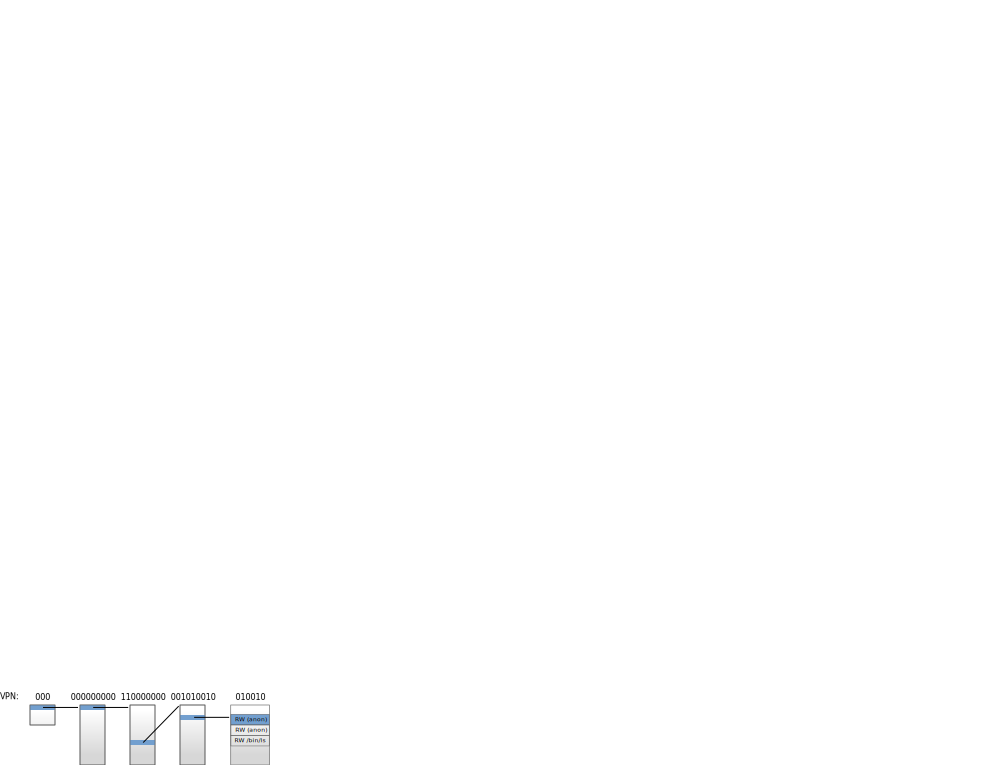
\includegraphics{figures/radix.pdf}
\caption{A radix tree containing both an anonymous mapping
  and a file mapping.  Blue indicates the path for looking up the 36-bit
  virtual page number shown in bits at the top of the figure.  The last
  level of the tree contains separate mapping metadata for each page.
}
\label{fig:radix}
\end{figure}

The index data structure of \vm resembles a hardware page table
structurally, storing mapping metadata in a fixed-depth radix tree,
where each level of the tree is indexed by nine (or fewer) bits of the
virtual page number (Figure~\ref{fig:radix}).  Like the linear array,
the radix tree supports only point queries (not range queries) and
iteration, but unlike the linear array, \vm can compress repeated
entries and lazily allocate the nodes of the radix tree.  Logically,
any node that would consist entirely of identical values is folded
into a single value stored in the parent node.  This continues up to
the root node of the tree, allowing the radix tree to represent vast
swaths of unused virtual address space with a handful of NULL values
and to set large ranges to identical values very quickly.  This
folding comes at a small cost: \code{mmap} operations that force
expansion of the radix tree may conflict with each other, even if
their regions do not ultimately overlap.  However, such conflicts are
rare.

To record each mapping, \vm stores a separate copy of the mapping metadata
in the radix tree for each page in the mapped range.  This differs
from a typical design that allocates a single metadata object
to represent the entire range of a mapping (e.g., virtual memory areas
in Linux).
Storing a separate copy of the metadata for each page makes sense in \vm
because the metadata is relatively small, and eliminating shared objects
avoids contention when a single mapping needs to be split or merged by
a subsequent \code{mmap} or \code{munmap} call.  Furthermore, the
mapping metadata object is designed so that it will initially be
identical for every page of a mapping, meaning that large mappings can
created efficiently and folded into just a few slots in the radix
tree's nodes.

Also unlike typical virtual memory system designs, \vm stores pointers
to physical memory pages in the mapping metadata for pages that have
been allocated.  This is easy to do in \vm because, modulo folding,
there is a single mapping metadata object for each page.  It's also
important to have this canonical representation of the physical memory
backing a virtual address space because of the way \vm handles TLB
shootdown (see \S\ref{sec:radixvm:tlb}).  This does increase the space
required by the radix tree, but, asymptotically, it's no worse than
the hardware page tables, and it means that the hardware page tables
themselves are cacheable memory that can be discarded by the OS to
free memory.

To keep the memory footprint of the radix tree in check, the OS must be
able to free nodes that no longer contain any valid mapping metadata.
To accomplish this without introducing contention, we leverage
\refcache to scalably track the number of used slots in each node.
When this count drops to zero, the radix tree can remove the node from
the tree and delete it.  Since \vm may begin using a node again before
\refcache reconciles the used slot count, nodes link to their children
using weak references, which allows the radix tree to revive nodes
that go from empty to used before \refcache deletes them, and to
safely detect when an empty child node has been deleted.

Collapsing the radix tree does introduce additional contention;
however, in
contrast with more eager garbage collection schemes, rapidly changing
mappings cannot cause the radix tree to rapidly delete and recreate
nodes.  Since a node must go unused for at least two \refcache epochs
before it is deleted, any cost of deleting or recreating it (and any
additional contention that results) is amortized.
\XXX[AC]{We don't actually implement this, but if we did, when we
analyze performance without \refcache, things would be even worse.
Might be worth mentioning.}

In contrast with more traditional balanced trees, using a radix tree
to manage address space metadata allows \vm to achieve perfect
scalability for operations on non-overlapping ranges of an address
space.  This comes at the cost of a potentially larger memory
overhead; however, address space layouts tend to exhibit good
locality and folding efficiently compresses large ranges, making radix
trees a good fit for a VM system.

\subsubsection{TLB shootdown}
\label{sec:radixvm:tlb}

One complication with scaling \code{mmap} or \code{munmap} operations
is the per-core hardware page translation cache, which requires
explicit notifications (``TLB shootdowns'') when a page mapping changes.
Because TLB shootdowns must be delivered to every CPU that may have
cached a page mapping that's being modified, and because hardware does not provide
information about which CPUs may have cached a particular mapping,
a conservative design must send TLB shootdown interrupts to all
CPUs using the same address space, which limits scalability.

\vm achieves better scalability for \code{mmap} and \code{munmap} by
keeping track of more precise information about the set of CPUs that
may have accessed a given mapping, as part of the mapping metadata.
With a software-filled TLB, the kernel can use TLB miss faults to track
exactly which CPUs have a given mapping cached.  When a later \code{mmap}
or \code{munmap} changes this mapping, it can deliver shootdowns
only to cores that have accessed this mapping.  On architectures
with hardware-filled TLBs such as the x86, our design achieves the
same effect using per-core page tables.  If a thread in an application
allocates, accesses, and frees memory on one core, with no other threads
accessing the same memory region, then \vm will perform no TLB shootdowns.

The obvious downside to this approach is the extra memory required for
per-core page tables.  We show in \S\ref{eval:memory} that this
overhead is small in practice compared to the total memory footprint
of an application, but for applications with poor partitioning, it may
be necessary for the application to provide hints about widely shared
regions so the kernel can share page tables (similar to Corey address
ranges~\cite{boyd-wickizer:corey}) or
the kernel could detect such regions automatically.  The kernel could
also reduce overhead by sharing page tables between small groups of
cores or by simply
discarding page table pages when memory is low.

\subsubsection{VM operations}

The POSIX semantics of VM operations can make a scalable implementation
of the operations challenging~\cite{clements:bonsai}. But, with the
components described above, the \vm implementation of the VM operations is
surprisingly straightforward.  The POSIX semantics that are challenging
are the ones that relate to ordering. For example, after the return
of an \code{munmap}, no thread should be able to access the unmapped
pages.  Similarly, after \code{mmap}, every thread that experiences a
\code{pagefault} should be able to access the mapped pages.  There is
also some
complexity in \code{pagefault} because it is not just a read operation:
it may have to allocate physical pages and modify the address space.

\vm primarily enforces correct ordering semantics by always locking,
from left to right, the radix tree entries for the region affected by
an operation.  Each slot in the radix tree (in both interior and leaf
nodes) reserves one bit for this purpose.  As a result, two concurrent
VM operations on overlapping ranges will serialize when locking the
leftmost overlapping page.

When locking a region that has not been expanded out to leaf nodes
yet, \vm acquires locks on the corresponding internal node slots instead.
When \vm expands the tree by allocating new nodes, it propagates the
lock bit to every entry in the newly allocated node, and unlocks the
parent interior node slot.  Releasing the lock clears the lock bits in the
newly allocated child node.  Tree traversal does not require locks
because it increments each node's reference count through a \refcache
weak reference.

An \code{mmap} invocation first locks the range being mapped.  As above,
if the leaf nodes for the range have already been allocated, \code{mmap}
locks the mapping metadata in the leaf nodes, and if not, it locks the
corresponding interior nodes.  If there are existing mappings within the
range, \code{mmap} unmaps them, as described later for \code{munmap}.
\code{mmap} then fills in mapping metadata for the new mapping (protection
level and flags arguments to \code{mmap}, as well as what backs this virtual
memory range, such as a file or anonymous memory).  If the mapping covers
an entire radix tree node, and the child nodes have not been allocated
yet, the radix tree collapses the mapping metadata into a single slot
in the interior of the tree.
Otherwise, \vm copies the mapping metadata into each leaf node entry in
the range.  Finally, \vm unlocks the range.  Like in other VM systems,
\code{mmap}
doesn't allocate any physical pages, but leaves that to \code{pagefault},
so that pages are allocated only when they are used.

A \code{pagefault} invocation traverses the radix tree to find the
mapping metadata for the faulting address, and acquires a lock on it.
It then allocates a physical page, if one has not been allocated yet, and
stores it in the mapping metadata.  Finally, \code{pagefault} fills in the
page table entry in the local core's page table, and adds the local core
number to the TLB shootdown list in the mapping metadata for that address.
\code{pagefault} then releases the lock and returns.

To implement \code{munmap}, \vm must clear mapping metadata from the
radix tree, clear page tables, invalidate TLBs, and free physical
pages.  \code{munmap} begins by locking the range being unmapped,
after which it can scan the region's metadata to gather references to
the physical pages backing the region, collect the set of cores that
have faulted pages in the region into their per-core page tables, and
clear each page's metadata.  It can then send inter-processor
interrupts to the set of cores it collected in the first step.  These
interrupts cause the remote cores (and the core running \code{munmap})
to clear the appropriate range in their per-core page table and
invalidate the corresponding local TLB entries.  Once all cores have
completed this shootdown process, \code{munmap} can safely release its
lock on the range and decrement the reference counts on the physical
pages that were unmapped.

Note that an invocation of \code{pagefault} on one core may concurrently
access a page that another core is in the process of unmapping,
but the mapping metadata lock makes this work out correctly: either
\code{pagefault} acquires the lock first or \code{munmap} does.  In the
first case, the page fault succeeds, which is okay since the pages must be
inaccessible only after \code{munmap} returns.  In the second case, the
\code{munmap} runs first and removes the mapping for the unmapped range
before releasing the locks. Then, \code{pagefault} will see that there
is no mapping for the faulting address and will halt the faulting thread.

\subsubsection{Discussion}

By combining \refcache for scalable reference counting, radix trees
for maintaining address space metadata, and per-core page tables for
precise TLB tracking and shootdown, \vm is able to execute concurrent
\code{mmap}, \code{munmap}, and \code{pagefault} operations on the
same address space in a way that shares cache lines only when two operations
manipulate overlapping regions and must be serialized.  With the right
data structures in place, \vm can achieve this with a straightforward
concurrency plan based on precise range locking.  We confirm that
\vm's design translates into scalable performance for non-overlapping
VM operations in \S\ref{sec:eval}.



\subsection{\fs: Conflict-free file system operations}

\XXX![AC]{This section may end up with redundant parts.  It may need
  more details about the design, or at least an intro that more
  strongly states that, unlike Refcache and RadixVM, \fs is all known
  techniques and \tool-guided elbow grease.}

\fs makes extensive use of existing techniques for scalable
implementations, such as per-core resource
allocation, double-checked locking, lock-free readers using
RCU~\cite{rcu:linux},
scalable reference counts using Refcache~\cite{clements:radixvm},
and seqlocks~\cite[\S6]{lameter:linuxsync}.  These techniques lead to
several common patterns, as follows; we illustrate the patterns with
example test cases from \tool{} that led us to discover these situations:


\paragraph{Layer scalability.}  \fs uses data structures that
themselves naturally satisfy the commutativity rule, such as linear
arrays, radix arrays~\cite{clements:radixvm}, and hash tables.  In
contrast with structures like balanced trees, these data
structures
typically share no cache lines when different elements are accessed
or modified.  For example, \fs stores the cached data pages for a given inode
using a radix array, so that concurrent reads or writes to different
file pages scale, even in the presence of operations
extending or truncating the file.
% , as long as they don't access the part
% of the file that's being extended or truncated.
Many operations also use this radix array to determine if some offset
is within the file's bounds without risking conflicts with operations
that change the file's size.

\XXX[AC]{Nir's book calls such data structures ``naturally parallel''
or something.}


\paragraph{Defer work.} Many kernel resources are shared,
such as files and pages, and must be freed when no longer referenced.
Typically, kernels release resources immediately, but this requires
eagerly tracking references to resources, causing
commutative operations that access the same resource to conflict.  Where
releasing a resource is not time-sensitive, \fs
uses Refcache~\cite{clements:radixvm} to batch reference count
reconciliation and zero detection.  This way, resources are eventually
released, but within each Refcache epoch commutative operations can be
conflict-free.

\XXX[AC]{Discuss crazy pipe hybrid reference counting scheme?}

\XXX[AC]{This seems uninteresting, and possibly false. \par
Batching sometimes enables absorption, when a resource gets reused within
a batch interval, thus requiring no non-scalable operations at all.
For instance, if one process closes the last open file descriptor for
a file, that file becomes eligible for eviction from the inode cache
(using Refcache weak references~\cite{clements:radixvm}).  However,
if another process re-opens the file on the same core, the inode can
be revived without any conflicting memory accesses.}

Some resources are artificially scarce, such as inode numbers in a typical
Unix file system.  When a typical Unix file system runs out of free
inodes, it must reuse an inode from a recently deleted file.  However,
the POSIX interface does not require that inode numbers be reused, only
that the same inode number is not used for two files at once.  Thus,
\fs never reuses inode numbers.  Instead, inode numbers are
generated by a monotonically increasing per-core counter, concatenated
with the core number that allocated the inode.  This allows \fs to defer
inode garbage collection for longer periods of time, and enables scalable
per-core inode allocation.


% \paragraph{Check before updating.}  Before updating any data structure,
% \fs first checks whether the data structure already contains the new
% value, and avoid any writes if so.  For example, the Linux file system
% always acquires a lock on an inode when truncating the file.  This means
% that concurrent truncate operations do not scale, even if the file
% is already empty.  \fs first checks the current length of the file,
% and avoids updating the length or acquiring any locks if the file is
% already at the right size.

% As another example, if one thread tries to create an existing file using
% \code{open(O_CREAT|O_EXCL)}, it should fail, but a na\"ive implementation
% might first acquire a lock to prepare for creating the file, and then
% check whether the file already exists.  This makes
% concurrent \code{open(O_CREAT|O_EXCL)} calls for an existing file name
% non-scalable.  \fs first checks whether the file already exists without
% modifying any cache lines, making these operations scale.

% \XXX[AC]{The above two examples are slightly off.  E.g., if I do two
% truncates and the first writes to the file length and the second reads
% that, that's sharing.  These are both idempotent updates, which is one
% of the few things we \emph{don't} do scalably.}

% As a final example, if two file names \code{a} and \code{b} point to the
% same inode, \code{rename(a, b)} should remove the directory entry for
% \code{a}, but it should not modify the directory entry for \code{b}, since
% it already points at the right inode.  By checking the directory
% entry for \code{b} before updating it, \fs allows \code{rename(a, b)}
% to scale with other operations that look up \code{b}.


\paragraph{Precede pessimism with optimism.} Many operations
in \fs have an optimistic check stage followed by a pessimistic update
stage, a generalized sort of double-checked locking.  The optimistic
stage checks conditions for the operation and returns immediately if
no updates are necessary (this is often the case for error returns,
but can also happen for success returns).  This stage does no writes
or locking, but because no updates are necessary, it is often easy to
make atomic.  If updates are necessary, the operation acquires
locks or uses lock-free protocols, re-verifies its conditions to
ensure atomicity of the update stage, and performs updates.  For
example, \code{lseek} first computes the new offset using a lock-free
read-only protocol and returns early if the new offset is invalid or
equal to the current offset.  Otherwise, \code{lseek} locks the file
offset, and re-computes the new offset to ensure consistency.

\code{rename} is similar.  If two file names \code{a} and \code{b}
point to the
same inode, \code{rename(a, b)} should remove the directory entry for
\code{a}, but it does not need to modify the directory entry for
\code{b}, since
it already points at the right inode.  By checking the directory
entry for \code{b} before updating it, \code{rename(a, b)} avoids
conflicts with other operations that look up \code{b}.


\paragraph{Don't read unless necessary.}  A common internal interface
in a file system implementation is a \code{namei} function that
checks whether a path name exists, and if so, returns the inode for
that path.
%
However, reading the inode is unnecessary
if the caller wants to know only whether a path name existed, such as
an \code{access(F_OK)} system call.  In particular, the \code{namei}
interface makes it impossible for concurrent \code{access(b, F_OK)}
and \code{rename(a, b)} operations to scale when \code{a} and \code{b}
point to different inodes, even though they commute.
\fs has a separate internal interface to check for existence of a
file name, without looking up the inode, which allows \code{access}
and \code{rename} to scale in such situations.


\subsection{Difficult-to-scale cases}

As \cref{fig:testcase-breakdown-sv6} illustrates, there are a few
(\pyexpr{mscan.xv6.shared} out of \pyexpr{mscan.ntestcases})
commutative test cases for
which \vm and \fs are not conflict-free.
%
The majority of these tests involve idempotent updates to internal
state, such as two \code{lseek} operations that both seek a file
descriptor to the same offset, or two anonymous \code{mmap} operations
with the same fixed base address and permissions.  While it is
possible implement these scalably, every implementation we considered
significantly impacted the performance of more common operations, so
we explicitly chose to favor common-case performance over total
scalability.  Even though we decided to forego scalability in these
cases, the commutativity rule and \tool forced us to consciously make
this trade-off.
%
\XXX[AC]{About 75\% are known idempotent.}

% Non-idempotent shared case list (incomplete):
% close_close_pe_5: Closing pipe writer (eager counting)
% close_read_pdc_0: Closing pipe writer, reading writer always EBADF
% close_write_pd8_0: Symmetric to close_read_pdc_0
% lseek_read_pad8_2: Reading nothing from two different offsets
% lseek_read_p8b6_3: Same as lseek_read_pad8_2
% mmap_mprotect_pf8_41: Making different read-only mappings read-only
%   (The mprotect is a no-op, but what it reads is modified)
% mmap_mprotect_pae_40: Same
% read_read_pce4_0: Two reads from a file full of zeroes
% read_write_pbb0_2: Reading nothing from different end-of-file offsets
% write_write_pff8_1: Writing to a pipe with no readers
%   (We could probably fix this one)
% write_write_pff8_2: Same
% write_write_pf78_1: Same

Other difficult-to-scale cases are more varied.  Several involve
reference counting of pipe file descriptors.  Closing the last file
descriptor for one end of a pipe must immediately affect the other
end; however, since there's generally no way to know a priori if a
\code{close} will close the pipe, a shared reference count is used in
some situations.  Other cases involve operations that return the same
result in either order, but for different reasons, such as two reads
from a file filled with identical bytes.

\XXX[AC]{fstest works around all radix tree expansion.  Is this
cheating?  That's actually an interesting case.}

\XXX[AC]{Summarize or something?}
